\documentclass[12pt,a4paper,oneside]{article}

\usepackage[margin=1in]{geometry}
\usepackage{setspace}
\usepackage[numbers,sort&compress]{natbib}
\usepackage[hidelinks]{hyperref}
\usepackage{amsmath,amssymb}
\usepackage{graphicx}
\usepackage{float}
\graphicspath{{figures/}{../figures/}}
\usepackage{booktabs}
\usepackage{multirow}
\usepackage{longtable}
\usepackage{array}
\usepackage{url}

\begin{document}
\onehalfspacing

\title{CSAF-Net: A Cross-Attention Gated Fusion Network for CNN--Vision Transformer Based Concrete Crack Detection}

\author{
Kirubanandhan K\\
\small Department of Software Engineering\\
\small Vellore Institute of Technology, India\\
\small 22MIS0634
}

\maketitle

\begin{abstract}
Concrete crack detection is an important task for structural inspection
and maintenance. This paper presents CSAF-Net, a hybrid deep learning
architecture that combines DenseNet-121 and Vision Transformer (ViT)
features through bidirectional cross-attention and learned gated fusion.
The model is evaluated on a balanced 4,000-image subset of SDNET2018.
Experiments compare CNN-only, ViT-only, feature concatenation, ungated
cross-attention, scalar-gated fusion, and the proposed gated fusion.
The full model achieves 86.00\% test accuracy, 87.00\% recall, and
86.14\% F1-score in the original run. Repeated runs are also examined
to assess variability. A separate synthetic wide-view localization
evaluation highlights the challenges of locating cracks in larger images.
\end{abstract}

\noindent\textbf{Keywords:}
Concrete crack detection, computer vision, DenseNet-121,
Vision Transformer, cross-attention, gated fusion.

\section{Introduction}

Cracks in concrete structures can indicate deterioration and may compromise structural durability if they remain undetected. Automated image-based crack detection offers a practical approach to inspecting concrete surfaces. However, crack appearance varies with lighting, surface texture, crack width, and background patterns, making reliable classification challenging.

Convolutional neural networks (CNNs) learn local visual features that are useful for identifying crack patterns. DenseNet-121 uses dense connections to facilitate feature reuse and information propagation \cite{densenet2017}. Vision Transformers (ViTs), in contrast, model relationships between image patches through self-attention \cite{vit2021,vaswani2017}. These complementary properties motivate the investigation of hybrid CNN–Transformer architectures for concrete crack detection.

This paper presents CSAF-Net, a CNN–Vision Transformer architecture that combines DenseNet-121 and ViT-Base/16 using bidirectional cross-attention and learned gated fusion. The proposed design projects both feature streams into a shared representation space, enables information exchange between the streams, and learns their relative contributions for binary crack classification.

The main contributions of this work are:
1. A dual-backbone architecture combining CNN-based local features and Transformer-based contextual representations.
2. A bidirectional cross-attention module followed by token-wise, channel-wise gated feature fusion.
3. An ablation study comparing individual backbones and alternative fusion strategies.
4. An exploratory wide-view localization evaluation that examines the limitations of applying a patch classifier to larger concrete images.



\section{Literature Survey}

Prior work on concrete crack detection includes image-based classification and segmentation approaches. SDNET2018 provides annotated concrete surface images for crack detection, while CrackVision investigates transfer learning for concrete crack classification \cite{sdnet2018,crackvision2025}. Attention-based methods have also been applied to concrete crack analysis and reinforced-concrete bridge inspection \cite{sarhadi2024,ruggieri2025}.

CNNs such as DenseNet extract local texture and edge information, whereas Vision Transformers model relationships among image patches \cite{densenet2017,vit2021,vaswani2017}. Hybrid CNN--Transformer models, cross-attention, and gated feature-fusion methods have also been investigated in other image-analysis domains \cite{effresnetvit2025,hussain2024,hajian2025,lee2025}. Related research covers solar-cell and tool-wear defect classification, lightweight attention, medical-image preprocessing, eye-disease diagnosis, and industrial defect detection \cite{abdelsattar2025,feng2025,alnamoly2024,rashid2025,eisentraut2025,zhang2025,rieck2025,lu2022}.

% ---------------------------------------------------------
% Literature Survey Table
% Place immediately after the Literature Survey paragraph
% ---------------------------------------------------------

\begin{longtable}{|p{2.5cm}|p{2.5cm}|p{3cm}|p{5cm}|}

\caption{Literature Survey and Relevance to CSAF-Net}
\label{tab:literature}\\

\hline
\textbf{Study} &
\textbf{Domain} &
\textbf{Method} &
\textbf{Finding and Relevance} \\
\hline
\endfirsthead

\multicolumn{4}{c}%
{{\tablename\ \thetable{} -- continued from previous page}}\\
\hline
\textbf{Study} &
\textbf{Domain} &
\textbf{Method} &
\textbf{Finding and Relevance} \\
\hline
\endhead

\hline
\multicolumn{4}{r}{Continued on next page}\\
\endfoot

\hline
\endlastfoot

Abdelsattar et al. (2025) &
Solar-cell defect detection &
Deep CNN classifiers &
Demonstrates automated visual defect classification; results can be sensitive to preprocessing and class imbalance. \\
\hline

Alkannad et al. (2025) &
Concrete crack detection &
CrackVision; pretrained CNN transfer learning &
Provides a direct concrete-crack classification baseline using transfer learning. \\
\hline

Alnamoly et al. (2024) &
Tomato-leaf disease classification &
FL-ToLeD; lightweight attention-augmented CNN &
Shows the use of attention to improve fine-grained visual classification. \\
\hline

Eisentraut et al. (2025) &
Tuberculosis detection from chest X-rays &
CNN with Gaussian-filter preprocessing &
Highlights the role of preprocessing in image-classification performance. \\
\hline

Feng et al. (2025) &
Tool-wear classification &
Improved DenseNet &
Provides a related application of densely connected features for fine-grained classification. \\
\hline

Hajian and Aramvith (2025) &
Remote-sensing super-resolution &
AERU-Net with edge recovery and attention &
Provides an example of attention-based feature refinement and learned gating. \\
\hline

Hussain and Shouno (2024) &
Medical-image segmentation &
MAGRes-UNet; multi-attention gated residual U-Net &
Provides a precedent for gated feature integration in visual recognition. \\
\hline

Lee et al. (2025) &
MRI-guided surgical planning &
Multi-view cross-attention &
Demonstrates cross-attention for exchanging information across feature views. \\
\hline

Lu et al. (2022) &
Internal defect detection in magnetic tiles &
MMFCNN with cross-attention fusion &
Provides an industrial-defect example of cross-attention-based feature fusion. \\
\hline

Rashid et al. (2025) &
Tomato-leaf disease detection &
MobileNetV3 with channel attention &
Illustrates channel attention in lightweight visual classification. \\
\hline

Rieck et al. (2025) &
Eye-disease diagnosis &
Transformer--CNN hybrid &
Provides cross-domain evidence for hybrid convolutional and Transformer representations. \\
\hline

Ruggieri et al. (2025) &
Reinforced-concrete bridge inspection &
Attention-augmented defect detector &
Directly relates attention mechanisms to structural-defect inspection. \\
\hline

Sarhadi et al. (2024) &
Concrete-crack segmentation &
Attention-based Swin U-Net &
Studies attention-based crack segmentation, a related task with a different output objective. \\
\hline

Venugopal et al. (2026) &
Thyroid diagnosis from ultrasound &
Multi-scale Vision Transformer with neural architecture search &
Provides an example of Transformer architecture optimization in medical imaging. \\
\hline

Zhang et al. (2025) &
Tomato-disease recognition &
Image dehazing with improved MobileNetV3 &
Provides a related example of preprocessing for visual classification. \\
\hline

\end{longtable}

\begin{figure*}[H]
    \centering
    \includegraphics[width=\textwidth]{csafnet_architecture_pictorial.png}
    \caption{Overview of CSAF-Net. DenseNet-121 and ViT-Base/16
    extract complementary features that interact through
    bidirectional cross-attention. The aligned representations
    are combined by a learned gate before binary crack classification.}
    \label{fig:csaf_architecture}
\end{figure*}

\section{Methods and Materials}

\begin{figure*}[H]
    \centering
    \includegraphics[width=\textwidth]{csafnet_architecture.png}
    \caption{Technical architecture of CSAF-Net, showing the DenseNet-121 and ViT-Base/16 branches, bidirectional cross-attention, learned gated fusion, and binary classification head.}
    \label{fig:csaf_architecture_technical}
\end{figure*}





\subsection{Overall Architecture}

CSAF-Net combines convolutional feature extraction and transformer-based
context modeling through bidirectional cross-attention and learned gated
fusion. The architecture consists of two pretrained backbones, feature
projection layers, a cross-attention fusion module, and a binary
classification head. DenseNet-121 extracts local visual representations,
while ViT-Base/16 captures relationships among image patches.

Given an input image $I \in \mathbb{R}^{3 \times 224 \times 224}$,
both backbones produce feature tokens that are projected into a shared
256-dimensional space. The pretrained backbone parameters are frozen
during training, while the projection layers and subsequent modules
are optimized for crack classification.

\subsection{Feature Extraction and Projection}

The DenseNet-121 feature extractor produces a feature map of size
$1024 \times 7 \times 7$. Flattening its spatial dimensions produces
49 tokens, each with 1024 channels. A linear projection maps these
tokens into a 256-dimensional feature space:
\begin{equation}
X_c = \operatorname{LN}(W_c T_c + b_c),
\end{equation}
where $T_c \in \mathbb{R}^{49 \times 1024}$ denotes the flattened
CNN features, $W_c$ and $b_c$ are learnable projection parameters,
and $\operatorname{LN}$ denotes layer normalization.

The ViT-Base/16 backbone produces one classification token and
196 patch tokens, each with 768 dimensions. The classification token
is removed, and the remaining patch tokens are projected as
\begin{equation}
X_v = \operatorname{LN}(W_v T_v + b_v),
\end{equation}
where $T_v \in \mathbb{R}^{196 \times 768}$ contains the patch
embeddings. Both projected representations have 256 feature
dimensions.

\subsection{Bidirectional Cross-Attention}

Cross-attention enables each feature branch to incorporate information
from the other branch. Let $X_c$ and $X_v$ denote the projected CNN
and ViT token sequences, respectively. The CNN-to-ViT attention
operation uses CNN tokens as queries and ViT tokens as keys and values:
\begin{equation}
A_c = \operatorname{LN}\left(
\operatorname{MHA}(X_c,X_v,X_v)+X_c
\right).
\end{equation}

In the reverse direction, ViT tokens query the CNN representations:
\begin{equation}
A_v = \operatorname{LN}\left(
\operatorname{MHA}(X_v,X_c,X_c)+X_v
\right).
\end{equation}

Both attention modules use eight heads, residual connections, and
layer normalization. The resulting sequences contain 49 and 196
tokens, respectively. To align them for fusion, the ViT-attended
sequence is adaptively average-pooled along the token dimension to
produce 49 tokens. Denote the aligned branches by $\widetilde{A}_c$
and $\widetilde{A}_v$.

\subsection{Learned Gated Fusion}

The aligned representations are concatenated along the feature
dimension and passed through a two-layer gating network:
\begin{equation}
G = \sigma\left(
W_2 \operatorname{ReLU}
\left(W_1[\widetilde{A}_c;\widetilde{A}_v]+b_1\right)
+b_2\right),
\end{equation}
where the gating network has dimensions $512 \rightarrow 256
\rightarrow 256$. The sigmoid function constrains gate values to
the interval $[0,1]$. The gate is input-conditioned and varies
across tokens and feature channels.

The final fused representation is
\begin{equation}
F = G \odot \widetilde{A}_c
  + (1-G) \odot \widetilde{A}_v,
\end{equation}
where $\odot$ denotes element-wise multiplication. This formulation
allows the network to assign different weights to the two attended
representations at each token and channel.

\subsection{Classification Head}

The fused token sequence is mean-pooled across its 49 tokens to
obtain a 256-dimensional vector:
\begin{equation}
z = \frac{1}{49}\sum_{i=1}^{49} F_i.
\end{equation}
The pooled vector is processed by a fully connected layer with
128 hidden units, ReLU activation, dropout with probability 0.3,
and a final linear layer that produces a single logit. Binary
cross-entropy with logits is used as the training objective.
The sigmoid function converts the output logit to a probability
during inference.

\section{Experimental Setup}

\subsection{Dataset and Data Partitioning}

Experiments were conducted using the wall subset of SDNET2018,
which contains images of cracked and uncracked concrete surfaces.
A balanced subset of 4,000 images was used, comprising 2,000
images per class. The dataset was partitioned into training,
validation, and test sets using a 70:15:15 ratio. The training
set contained 2,800 images, while the validation and test sets
contained 600 images each. Each partition was balanced, with
equal numbers of cracked and uncracked images.




Representative examples from the dataset used in this study are shown
in Fig.~\ref{fig:dataset_samples}, illustrating concrete surface images
from the crack and non-crack classes.

\begin{figure}[H]
    \centering
    \includegraphics[width=0.85\columnwidth]{figures/dataset_samples.png}
    \caption{Representative dataset images. Top: non-crack examples; bottom: crack examples.}
    \label{fig:dataset_samples}
\end{figure}

The dataset preparation script used Python's random-number
generator with seed 42 and a maximum selection limit of 2,000
images per class. The existing dataset split was retained for
the reported experiments.
\subsection{Image Preprocessing}

All input images were resized to $224 \times 224$ pixels.
Images were converted to tensors and normalized using the
ImageNet channel-wise mean
$(0.485, 0.456, 0.406)$ and standard deviation
$(0.229, 0.224, 0.225)$. Random horizontal flipping was
applied to training images only. Validation and test images
underwent resizing and normalization without random
augmentation.

\subsection{Training Configuration}

The models were trained for five epochs with a batch size
of eight. AdamW was used as the optimizer with a learning
rate of $10^{-4}$. Binary cross-entropy with logits served
as the loss function. The DenseNet-121 and ViT backbone
parameters were frozen, while the projection layers, fusion
module, and classification head were trainable. The checkpoint
with the highest validation F1-score was saved and reloaded
for evaluation on the held-out test set.

The experiments were implemented in Python 3.9.6 using
PyTorch 2.8.0 and Torchvision 0.23.0. The development
environment reported availability of Apple's Metal
Performance Shaders (MPS) backend.
\begin{figure}[H]
    \centering
    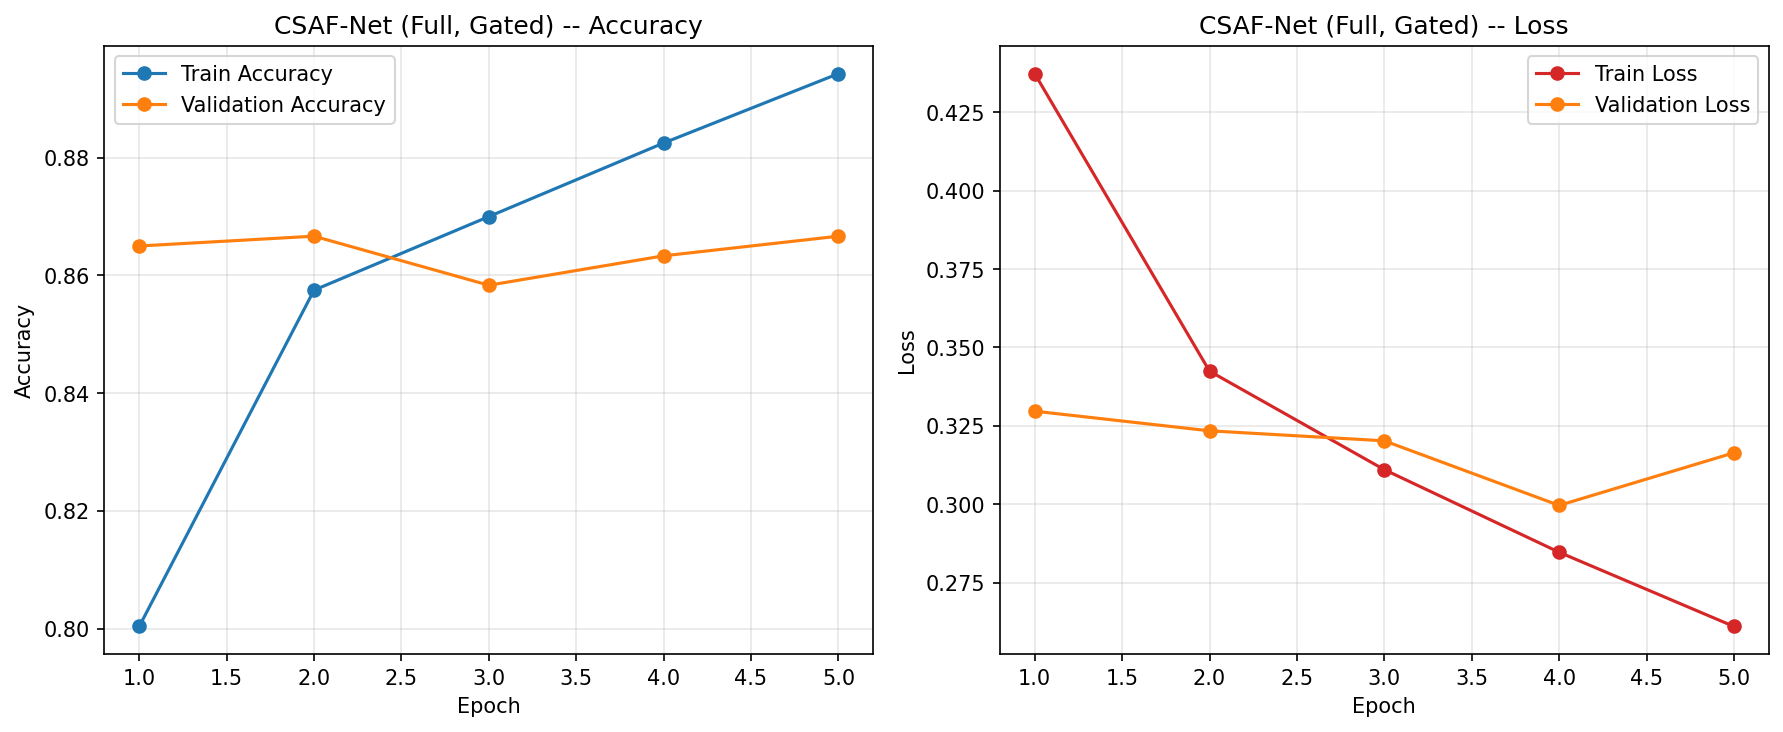
\includegraphics[width=0.9\columnwidth]{training_curves.png}
    \caption{Training and validation curves for the proposed
    CSAF-Net model.}
    \label{fig:training_curves}
\end{figure}

\subsection{Evaluation Metrics}

Classification performance was evaluated using accuracy,
precision, recall, and F1-score. Accuracy measures the
proportion of correctly classified images. Precision measures
the proportion of predicted crack-positive images that are
actually cracked, while recall measures the proportion of
cracked images correctly detected. F1-score is the harmonic
mean of precision and recall.

These metrics are reported for all six classification
variants to compare the individual backbones and the
contribution of the fusion strategies.

\section{Results and Discussion}

\subsection{Classification Ablation Study}

Table~\ref{tab:ablation} presents the test-set performance of
six model variants. The CNN-only and ViT-only models provide
single-backbone baselines. Feature concatenation, ungated
cross-attention, and scalar-gated fusion are evaluated to
investigate alternative feature-combination strategies.

\begin{table}[H]
\centering
\caption{Classification Results on the Held-Out Test Set}
\label{tab:ablation}
\small
\setlength{\tabcolsep}{4pt}
\begin{tabular}{lrrrr}
\toprule
\textbf{Model} & \textbf{Acc.} & \textbf{Prec.} &
\textbf{Rec.} & \textbf{F1} \\
\midrule
CNN-only & 75.33 & 79.46 & 68.33 & 73.48 \\
ViT-only & 82.83 & 85.82 & 78.67 & 82.09 \\
Concatenation & 84.17 & 84.51 & 83.67 & 84.09 \\
Ungated cross-attention & 85.83 & 89.09 & 81.67 & 85.22 \\
Scalar-gated fusion & 85.67 & 86.64 & 84.33 & 85.47 \\
\textbf{Full CSAF-Net} & \textbf{86.00} & 85.29 &
\textbf{87.00} & \textbf{86.14} \\
\bottomrule
\end{tabular}

\vspace{1mm}
\parbox{\columnwidth}{\footnotesize
All metrics are percentages.}
\end{table}


The full CSAF-Net model achieved 86.00\% accuracy, 87.00\%
recall, and an F1-score of 86.14\% in the original run.
Compared with the CNN-only baseline, the F1-score increased
by 12.66 percentage points. The ViT-only baseline also
outperformed the CNN-only model, indicating that transformer
features provide useful information for this classification task.

Feature concatenation achieved an F1-score of 84.09\%,
while ungated cross-attention and scalar-gated fusion achieved
85.22\% and 85.47\%, respectively. The full model produced
the highest F1-score among the six original runs, although
ungated cross-attention achieved the highest precision at
89.09\%.

These results show that the proposed combination of
bidirectional cross-attention and learned gating is promising
for crack classification. However, the single-run ablation
results alone do not establish that the learned gate produces
a statistically significant improvement over alternative
fusion strategies.
\begin{figure}[H]
    \centering
    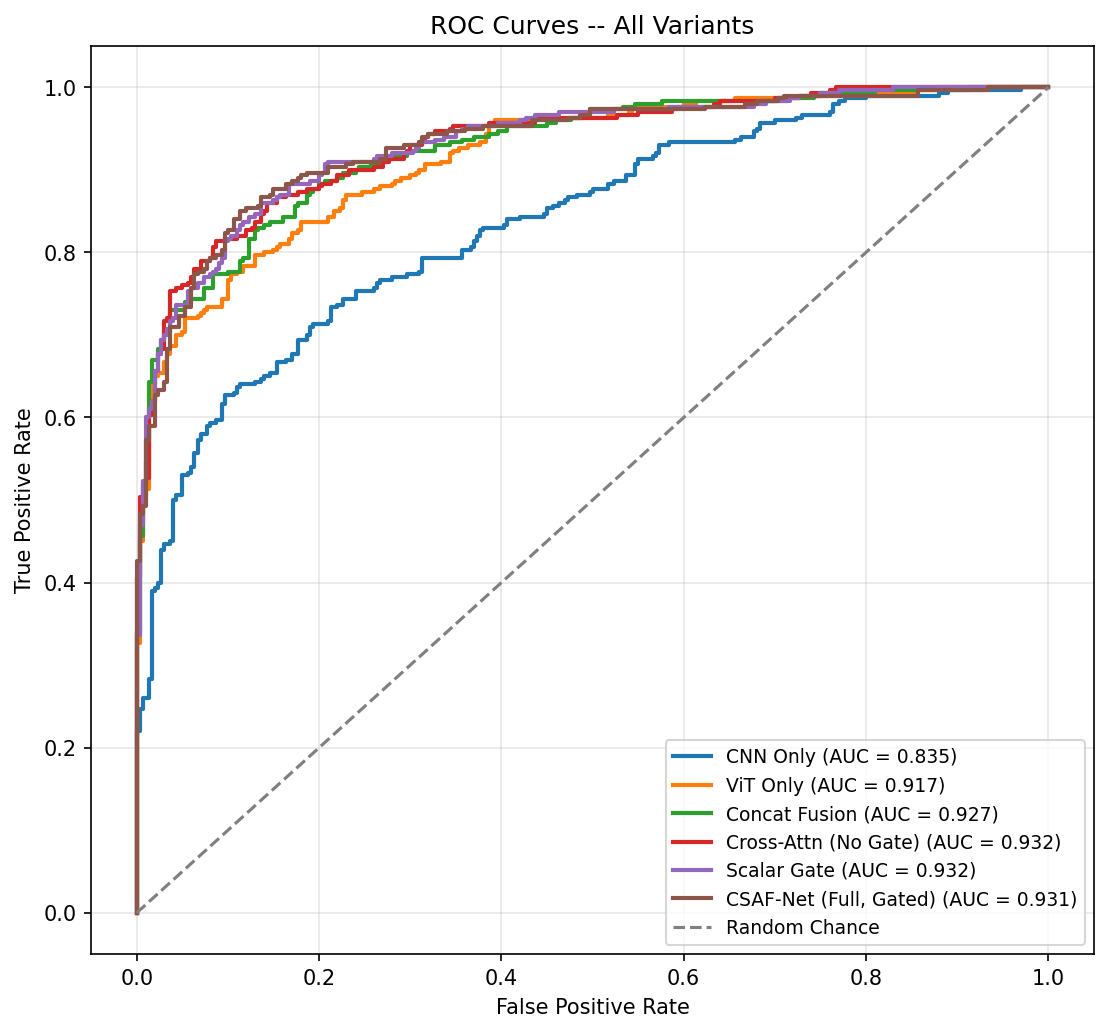
\includegraphics[width=\columnwidth]{roc_curves.png}
    \caption{Receiver operating characteristic (ROC) curves
    for the evaluated classification variants.}
    \label{fig:roc_curves}
\end{figure}

\begin{figure}[H]
    \centering
    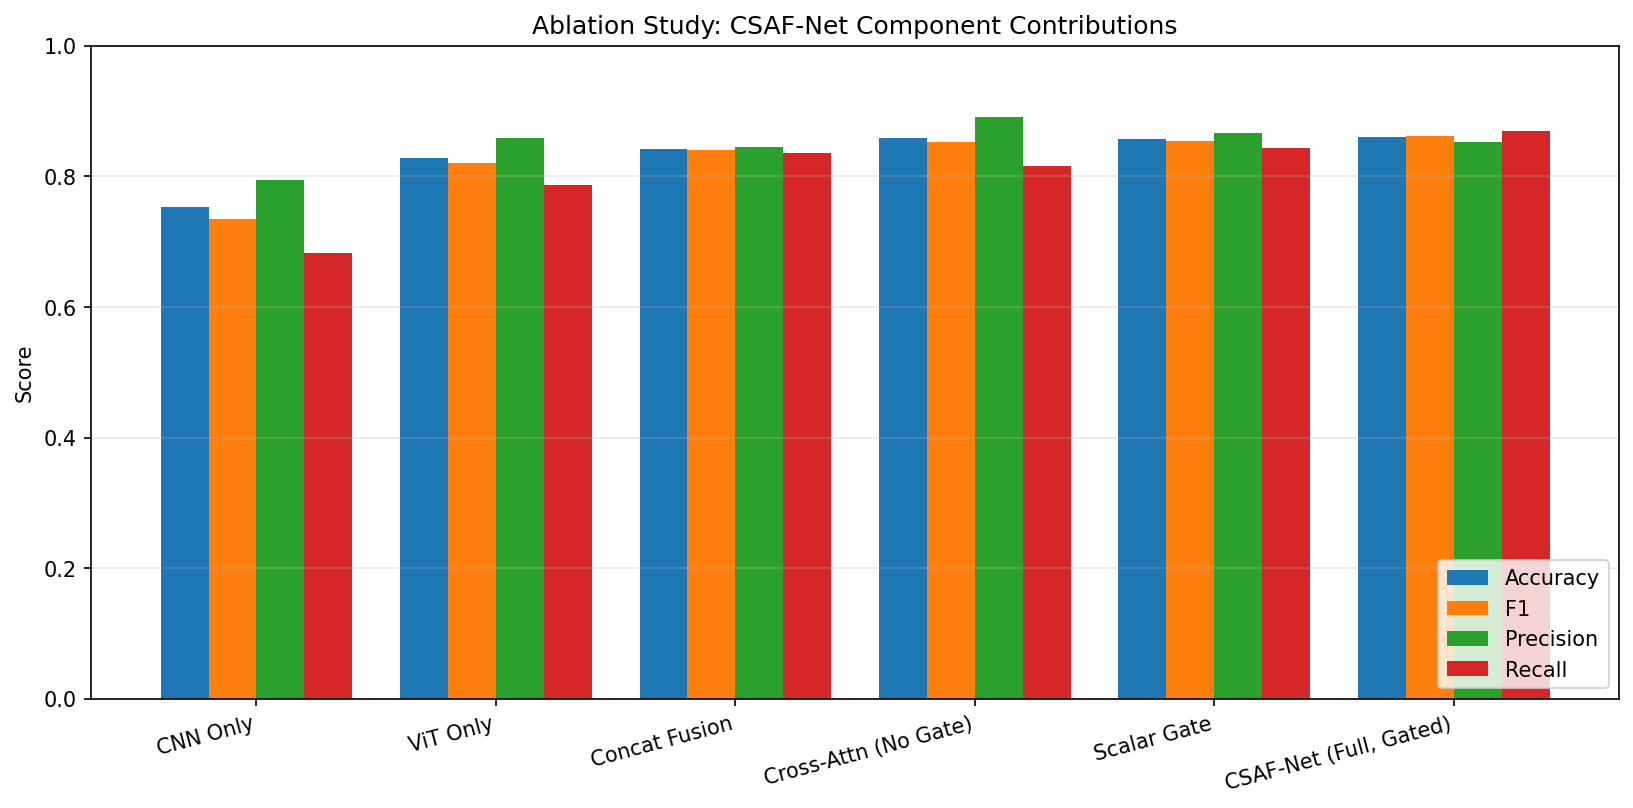
\includegraphics[width=0.88\columnwidth]{ablation_comparison.png}
    \caption{Comparison of accuracy, F1-score, precision,
    and recall across the six classification variants.}
    \label{fig:ablation_comparison}
\end{figure}

\begin{figure}[H]
    \centering
    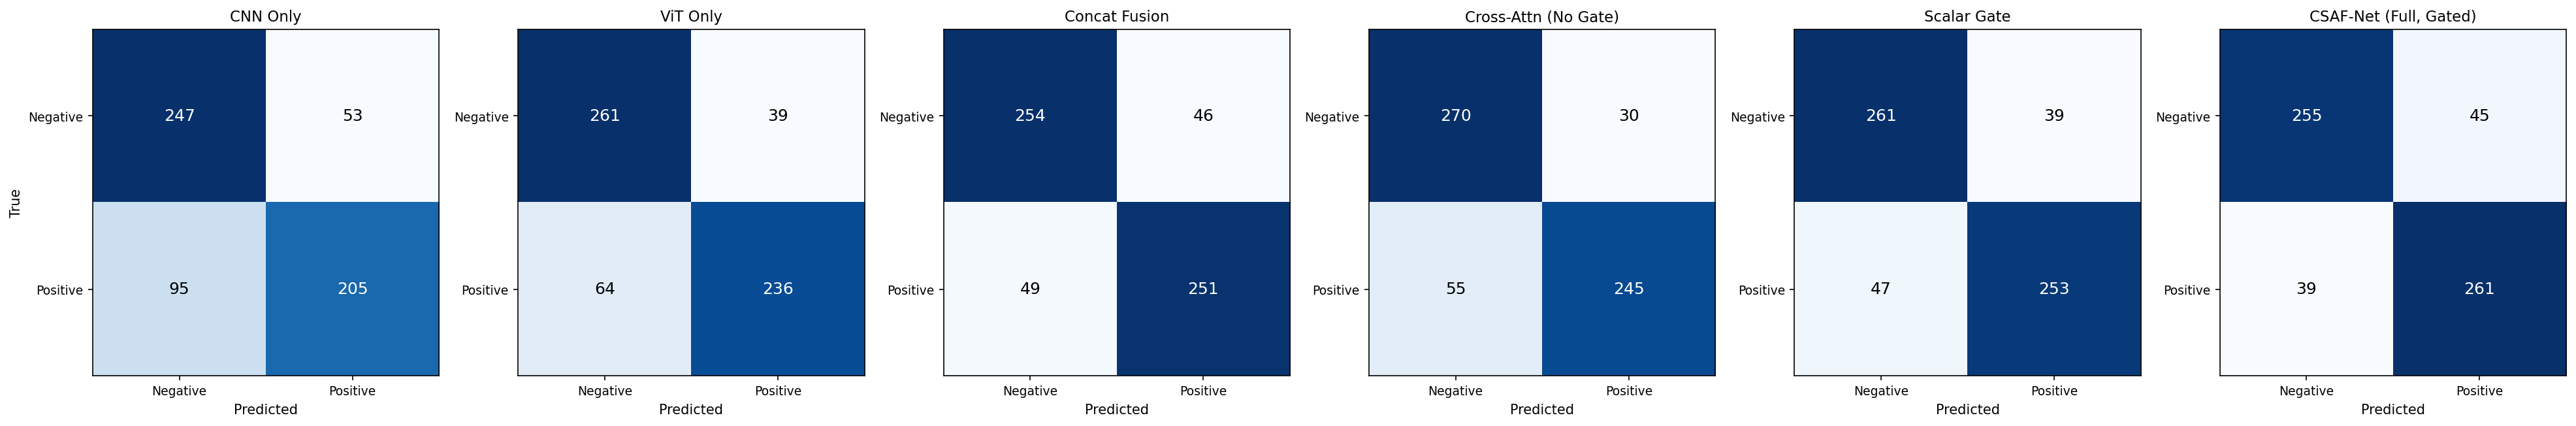
\includegraphics[width=\columnwidth]{confusion_matrices.png}
    \caption{Confusion matrices for the evaluated classification
    variants on the held-out test set.}
    \label{fig:confusion_matrices}
\end{figure}
\subsection{Repeated-Run Analysis}

To examine variability, the full CSAF-Net, scalar-gated
fusion, and ungated cross-attention variants were evaluated
in three runs each, consisting of the original run and two
additional reruns. Table~\ref{tab:repeated} reports the
mean and sample standard deviation.

\begin{table}[H]
\centering
\caption{Repeated-Run Classification Results}
\label{tab:repeated}
\scriptsize
\setlength{\tabcolsep}{2pt}
\begin{tabular}{@{}lrrrr@{}}
\toprule
Model & Acc. & Prec. & Rec. & F1 \\
\midrule
Full CSAF-Net
& $85.78 \pm 0.54$ & $85.64 \pm 1.26$
& $86.00 \pm 1.00$ & $85.81 \pm 0.46$ \\
Scalar-gated
& $85.94 \pm 0.63$ & $87.09 \pm 2.87$
& $84.56 \pm 2.34$ & $85.75 \pm 0.30$ \\
Ungated cross-attn.
& $86.06 \pm 0.38$ & $89.24 \pm 0.37$
& $82.00 \pm 1.20$ & $85.46 \pm 0.52$ \\
\bottomrule
\end{tabular}

\parbox{\columnwidth}{\footnotesize
Values are mean $\pm$ sample standard deviation in
percentages over three runs.}
\end{table}


Across the three runs, full CSAF-Net had the highest mean
recall and a marginally higher mean F1-score than the other
two fusion variants. Ungated cross-attention achieved the
highest mean precision and accuracy. The differences in mean
F1-score were small, so these results should be interpreted
as observed trends rather than evidence of statistically
significant superiority. The original run's random seed was
not recorded, and only three runs were available for each
variant.

\subsection{Wide-View Crack Localization}

In addition to image-level classification, a separate synthetic
wide-view benchmark was used to investigate whether the
classification model could localize cracks within larger images.
The benchmark used $900 \times 900$ scenes containing either a
crack region or no crack region. Crack regions were generated
with sizes between 150 and 300 pixels. A sliding-window
procedure used $224 \times 224$ crops with a stride of 56 pixels.
A predicted window was considered localized when its intersection
over union (IoU) with the reference box exceeded 0.3.

The detection threshold was selected using validation scenes
under a constraint of at most 0.2 false-positive boxes per
clean scene. The selected threshold for the single CSAF-Net
model was 0.995. On the held-out synthetic test benchmark,
the model localized 45 of 100 crack-containing scenes, giving
a scene-level localization recall of 45\% (95\% Wilson
confidence interval: approximately 35.6--54.8\%). The mean
IoU among localized cracks was 0.541, with 0.14 false-positive
boxes per clean scene. Scene-level precision was 80.4\% and
scene-level F1-score was 57.7\%.

A secondary threshold analysis evaluated a threshold of 0.992
on the same held-out scenes. It localized 52 of 100 crack
scenes (52\%), with mean IoU of 0.536 and 0.52 false-positive
boxes per clean scene. Although recall increased, the false-
positive rate exceeded the predefined validation budget, and
scene-level F1-score decreased to 55.3\%. Therefore, the
validation-selected threshold of 0.995 is retained as the
primary result; the 0.992 analysis is reported only as a
secondary operating-point comparison.

These findings indicate that high image-level classification
performance does not automatically translate into reliable
localization in wide-view images. The synthetic benchmark is
limited in its scene construction and should not be interpreted
as evidence of equivalent performance on unrestricted real-world
images.
\section{Limitations}

This study has several limitations. First, the classification
experiments use a balanced subset of SDNET2018 wall images.
Evaluation on additional datasets and real-world acquisition
conditions is necessary to establish cross-domain generalization.

Second, the repeated-run analysis includes only three runs for
each of the three fusion variants. The observed differences in
mean F1-score are small and do not establish statistically
significant superiority of the proposed gating mechanism.
Additional repeated experiments and controlled statistical
comparisons would provide stronger evidence.

Third, the wide-view localization benchmark uses synthetic
$900 \times 900$ scenes and predefined crack regions. Its results
may not reflect the complexity of real structures, including
variable lighting, surface texture, perspective, and crack
geometry. The localization pipeline relies on sliding-window
classification rather than a model trained explicitly for
object detection or pixel-level segmentation. Consequently,
the reported localization performance should be interpreted
within the scope of the synthetic benchmark.

Finally, the dataset preparation script fixes the random seed
but does not sort the source filenames before shuffling.
Consequently, reproducing the exact split may depend on the
ordering returned by the file system. The script does not save
a split manifest; therefore, the generated dataset and its
file assignments should be retained to reproduce the reported
experiments.

\section{Conclusion}

This paper presented CSAF-Net, a hybrid architecture that
combines DenseNet-121 and ViT-Base/16 representations using
bidirectional cross-attention and learned gated feature fusion
for concrete crack classification. On the evaluated
4,000-image SDNET2018 wall subset, the original run achieved
86.00\% test accuracy, 87.00\% recall, and an F1-score of
86.14\%. Among the six original classification variants,
the full model achieved the highest accuracy, recall, and
F1-score in that run.

Across repeated runs, the full model achieved the highest
mean recall and a marginally higher mean F1-score than the
scalar-gated and ungated cross-attention variants. These
differences do not establish statistically significant
superiority over the alternatives.

The separate synthetic wide-view evaluation revealed a
remaining challenge: image-level classification performance
does not guarantee reliable crack localization in larger
scenes. Future work will focus on broader cross-dataset
evaluation, additional repeated experiments, improved
localization methods, and validation on real-world images
with reliable ground-truth annotations.

\bibliographystyle{IEEEtran}
\bibliography{references}

\end{document}
